\documentclass[a3paper,14pt]{extarticle}
\usepackage[utf8]{inputenc}
\usepackage{extsizes}
\usepackage[T2A]{fontenc}
\usepackage[english,russian]{babel} 
\usepackage[left=15mm, top=25mm, right=15mm, bottom=25mm, nohead, nofoot]{geometry}
\usepackage{graphicx}
\usepackage{nicefrac}
\usepackage{amsmath,amsfonts,amssymb} % математический пакет
\usepackage{fancybox,fancyhdr} % хедер и футер
\pagestyle{fancy}
\fancyhf{}
\fancyhead[L]{Практическая линейная алгебра}
\fancyhead[R]{Овчинников Павел}
\fancyfoot[C]{\thepage}
\setcounter{page}{1}
\headsep=10mm 
\usepackage{hyperref}

\begin{document}
\section*{\centering Лабораторная работа №2}
Выберем 4 числа $a=5$, $b=3$, $c=2$, $d=7$ --- ни одно из них не равно $0$ или $\pm1$.
\subsection*{\centering Задание №1. Imagine Dragons}
Придумать — задачка интересная, конечно, но лучше всё же по возможности искать матрицы вычислительным путём. \\[0.5em]
1. Начнём с симметрии плоскости относительно прямой. Для этого нарисуем прямую $y=5x$ на плоскости и выберем две пары точек, где в каждой из пар отрезок, соединяющий их, образует прямой угол с $y=5x$ --- преобразование одной из точек каждой пары в другую и будет отражением плоскости относительно прямой.
\begin{figure}[h]
    \centering
    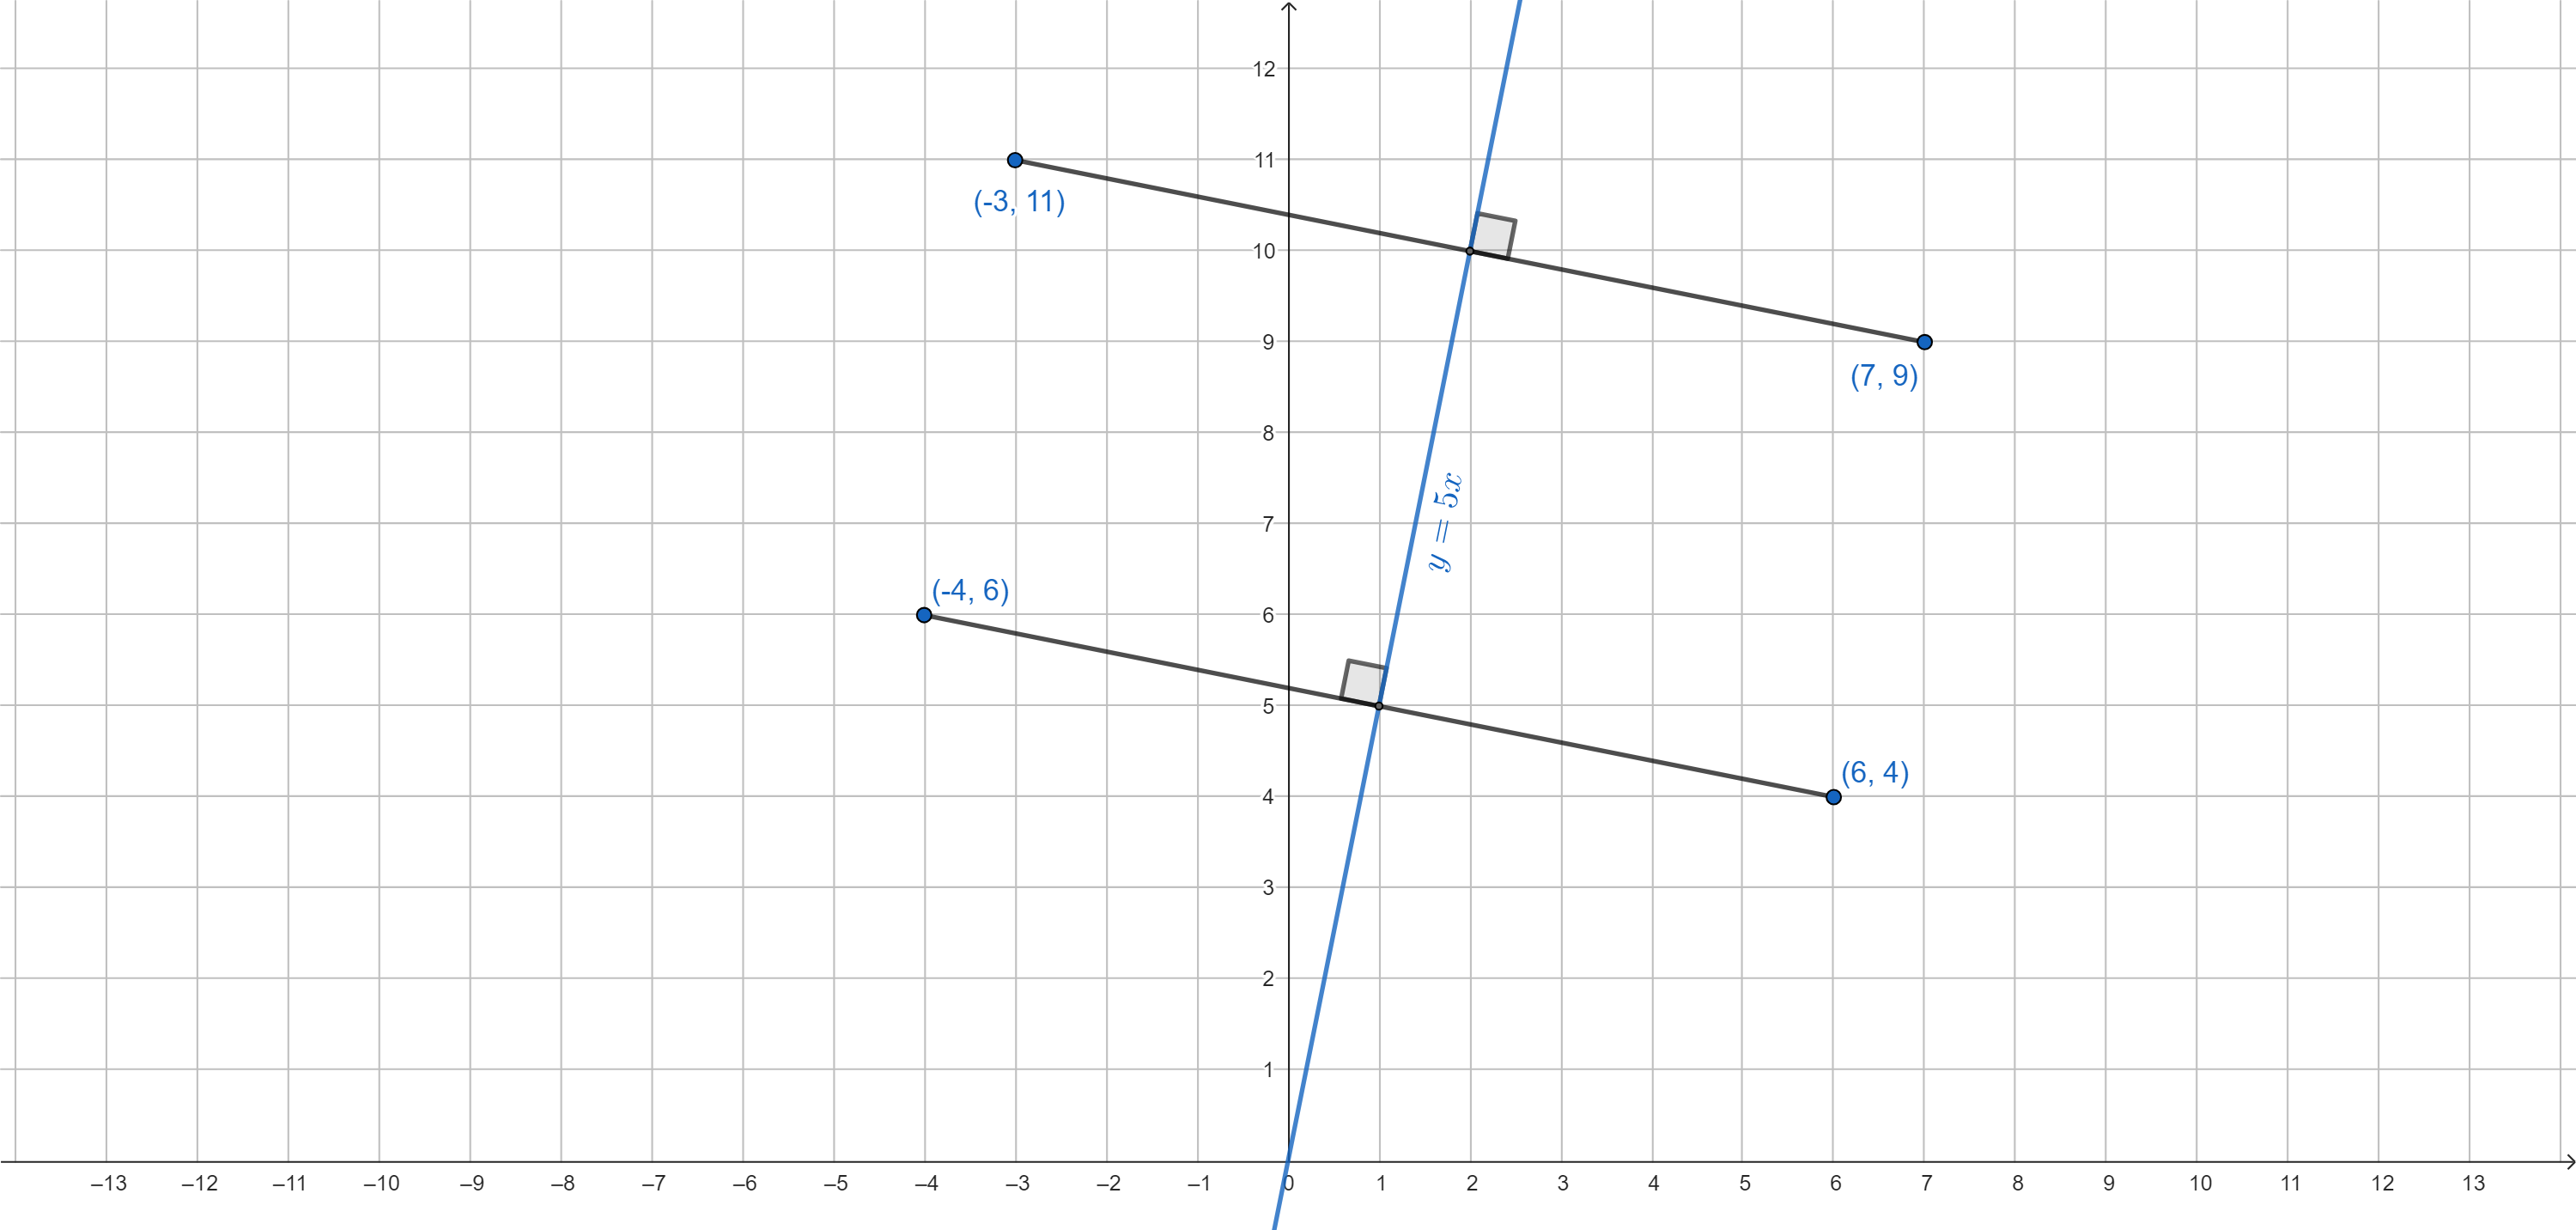
\includegraphics[width=0.8\textwidth]{task1.png}
\end{figure} \\
Теперь координаты точек в каждой из пар точек можно представить как действие линейного отображения на координаты другой точки в каждой из пар. Получим:
$$\begin{bmatrix}
        x_1 & x_2 \\ x_3 & x_4
    \end{bmatrix}\begin{bmatrix}
        7 \\ 9
    \end{bmatrix} = \begin{bmatrix}
        -3 \\ 11
    \end{bmatrix} \Rightarrow \begin{cases}
        7x_1+9x_2 = -3 \\ 7x_3+9x_4 = 11
    \end{cases}$$$$\begin{bmatrix}
        x_1 & x_2 \\ x_3 & x_4
    \end{bmatrix}\begin{bmatrix}
        6 \\ 4
    \end{bmatrix} = \begin{bmatrix}
        -4 \\ 6
    \end{bmatrix} \Rightarrow \begin{cases}
        6x_1+4x_2 = -4 \\ 6x_3+4x_4 = 6
    \end{cases}$$
Скомпонуем системы так, чтобы в одной системе были только $x_1$ и $x_2$, а в другой в то же время $x_3$ и $x_4$:
$$\begin{cases}
        7x_1 + 9x_2 = -3 \\ 6x_1 + 4x_2 = -4
    \end{cases} \Leftrightarrow \begin{cases}
        7x_1 + 9x_2 = -3 \\ x_2 = -1 - \nicefrac{3}{2}\;x_1
    \end{cases} \Leftrightarrow \begin{cases}
        -\nicefrac{13}{2}\;x_1 = 6 \\ x_2 = -1 - \nicefrac{3}{2}\;x_1
    \end{cases} \Leftrightarrow \begin{cases}
        x_1 = -\nicefrac{12}{13} \\ x_2 = -1 + \nicefrac{18}{13}
    \end{cases} \Rightarrow \begin{cases}
        x_1 = -\nicefrac{12}{13} \\ x_2 = \nicefrac{5}{13}
    \end{cases}$$
$$\begin{cases}
        7x_3 + 9x_4 = 11 \\ 6x_3 + 4x_4 = 6
    \end{cases} \Leftrightarrow \begin{cases}
        7x_3 + 9x_4 = 11 \\ x_3 = 1 - \nicefrac{2}{3}\;x_4
    \end{cases} \Leftrightarrow \begin{cases}
        -\nicefrac{13}{3}\;x_4 = 4 \\ x_3 = 1 - \nicefrac{2}{3}\;x_4
    \end{cases} \Leftrightarrow \begin{cases}
        x_4 = \nicefrac{12}{13} \\ x_3 = 1 - \nicefrac{8}{13}
    \end{cases} \Rightarrow \begin{cases}
        x_3 = \nicefrac{5}{13} \\ x_4 = \nicefrac{12}{13}
    \end{cases}$$
Итак, вычислив $x_1$, $x_2$, $x_3$ и $x_4$, получаем матрицу отражения плоскости относительно прямой $y=5x$:
$$A = \begin{bmatrix}
    \nicefrac{-12}{13} & \nicefrac{5}{13} \\ \nicefrac{5}{13} & \nicefrac{12}{13}
\end{bmatrix}$$
\textbf{\textit{Рубрика «наблюдения»}:} дроби, сформированные в матрице --- не что иное, как стороны прямоугольного треугольника с гипотенузой, равной единице. К квадрату коэффициента $k$ прямой $y = kx$ ищется ближайшее число $n$, которое в сумме с квадратом коэффициента даст квадрат числа $n+1$, т.е. $(n+1)^2=n^2+k^2$, и с этими числами формируются дроби $\nicefrac{k}{n+1}$ и $\nicefrac{n}{n+1}$ в матрице, причём на главной диагонали встанет дробь $\nicefrac{n}{n+1}$ с разными знаками, а на побочной --- дробь $\nicefrac{k}{n+1}$ с коэффициентом $k$. В таком случае катеты по сути отражаются оси $Ox$ и $Oy$, а гипотенуза --- единичный отрезок.\pagebreak

\noindent 2. Подобный алгоритм применим и для расчёта этого отображения. Нам понадобятся две точки по обе стороны от прямой $y=3x$: точка $(-2, 4)$, которая преобразуется линейным отображением в точку $(1, 3)$, и точка $(5, 5)$, которая под действием линейного отображения станет точкой $(2, 6)$. И получим следующие матричные выражения и системы, образованные ими:
$$\begin{bmatrix}
    x_1 & x_2 \\ x_3 & x_4
\end{bmatrix}\begin{bmatrix}
    -2 \\ 4
\end{bmatrix} = \begin{bmatrix}
    1 \\ 3
\end{bmatrix} \Rightarrow \begin{cases}
    -2x_1+4x_2 = 1 \\ -2x_3+4x_4 = 3
\end{cases}$$$$\begin{bmatrix}
    x_1 & x_2 \\ x_3 & x_4
\end{bmatrix}\begin{bmatrix}
    5 \\ 5
\end{bmatrix} = \begin{bmatrix}
    2 \\ 6
\end{bmatrix} \Rightarrow \begin{cases}
    5x_1+5x_2 = 2 \\ 5x_3+5x_4 = 6
\end{cases}$$
Точно так же перекомпонуем системы и найдём их решения в $x_1$, $x_2$, $x_3$ и $x_4$:
$$\begin{cases}
    -2x_1+4x_2 = 1 \\ 5x_1+5x_2 = 2
\end{cases} \Leftrightarrow \begin{cases}
    -2x_1+4x_2 = 1 \\ x_2 = 1-7x_1
\end{cases} \Leftrightarrow \begin{cases}
    x_1 = \nicefrac{1}{10} \\ x_2 = 1-7x_1
\end{cases} \Rightarrow \begin{cases}
    x_1 = \nicefrac{1}{10} \\ x_2 = \nicefrac{3}{10}
\end{cases}$$
$$\begin{cases}
    -2x_3+4x_4 = 3 \\ 5x_3+5x_4 = 6
\end{cases} \Leftrightarrow \begin{cases}
    -2x_3+4x_4 = 3 \\ x_4 = 3-7x_3
\end{cases} \Leftrightarrow \begin{cases}
    x_3 = \nicefrac{3}{10} \\ x_4 = 3-7x_3
\end{cases} \Rightarrow \begin{cases}
    x_3 = \nicefrac{3}{10} \\ x_4 = \nicefrac{9}{10}
\end{cases}$$
Итак, вычислив $x_1$, $x_2$, $x_3$ и $x_4$, получаем матрицу отображения плоскости в прямую $y=3x$:
$$B=\begin{bmatrix}
    \nicefrac{1}{10} & \nicefrac{3}{10} \\ \nicefrac{3}{10} & \nicefrac{9}{10}
\end{bmatrix}$$\,\\[0.5em]
3. Матрица поворота на $\theta$ градусов в общем виде выглядит как матрица с $\cos\theta$ на главной диагонали и с разными по знаку $\sin\theta$ на побочной диагонали. Тогда линейное отображение, поворачивающее плоскость на $20^\circ$ против часовой стрелки, будет выглядеть так:
$$C = \begin{bmatrix}
    \cos20^\circ & -\sin20^\circ \\ \sin20^\circ & \cos20^\circ
\end{bmatrix}$$\,\\[0.5em]
4. Центральная симметрия преобразовывает каждую точку плоскости из координаты $(x, y)$ в $(-x, -y)$. Нетрудно догадаться, какая \underline{единственная} для такой симметрии матрица существует:
$$D = \begin{bmatrix}
    -1 & 0 \\ 0 & -1
\end{bmatrix}$$\,\\[0.5em]
5. Отображение $F$, которое выполняет последовательно отражение и поворот, можно представить как произведение двух матриц, выполняющих эти действия. Притом важен порядок: ввиду того, что сначала выполняется отражение, а затем поворот, то к вектору применяется сначала $A$, а затем $\tilde{E}$ (новая матрица поворота, которая будет описана ниже), которое как бы оборачивает результат $Av$. Мы будем использовать матрицу из п.1 и немного изменённую матрицу из п.3, где вместо $20^\circ$ будет стоят $70^\circ$, а знаки у синусов будут изменены, т.к. поворот осуществляется по часовой стрелке:
$$\tilde{E} = \begin{bmatrix}
    \cos70^\circ & \sin70^\circ \\ -\sin70^\circ & \cos70^\circ
\end{bmatrix}$$
$$F = \tilde{E}A = \begin{bmatrix}
    \cos70^\circ & \sin70^\circ \\ -\sin70^\circ & \cos70^\circ
\end{bmatrix}\begin{bmatrix}
    \nicefrac{-12}{13} & \nicefrac{5}{13} \\ \nicefrac{5}{13} & \nicefrac{12}{13}
\end{bmatrix} = \begin{bmatrix}
    \nicefrac{-12}{13}\cos70^\circ + \nicefrac{5}{13}\sin70^\circ &
    \nicefrac{5}{13}\cos70^\circ + \nicefrac{12}{13}\sin70^\circ \\
    \nicefrac{12}{13}\sin70^\circ + \nicefrac{5}{13}\cos70^\circ &
    \nicefrac{-5}{13}\sin70^\circ + \nicefrac{12}{13}\cos70^\circ
\end{bmatrix}$$
Итак, мы получили отображение, которое сначала отражает плоскость относительно прямой $y = 5x$, а затем поворачивает её на $70^\circ$ по часовой стрелке.\\[1.5em]
6. Заметим, что когда мы говорим о прямых $x=0$ и $y = 0$, то речь заходит об осях $Ox$ и $Oy$ и стандартном базисе $\left\{(1, 0), (0, 1)\right\}$. Зная координаты начальных векторов и конечные векторы $(1, 5)$ и $(1, 3)$, в которые будут преобразованы начальные, мы можем найти матрицу отображения:
$$\begin{bmatrix}
    x_1 & x_2 \\ x_3 & x_4
\end{bmatrix}\begin{bmatrix}
    1 \\ 0
\end{bmatrix} = \begin{bmatrix}
    1 \\ 5
\end{bmatrix} \Rightarrow \begin{cases}
    x_1 = 1 \\ x_3 = 5
\end{cases}$$
$$\begin{bmatrix}
    x_1 & x_2 \\ x_3 & x_4
\end{bmatrix}\begin{bmatrix}
    0 \\ 1
\end{bmatrix} = \begin{bmatrix}
    1 \\ 3
\end{bmatrix} \Rightarrow \begin{cases}
    x_2 = 1 \\ x_4 = 3
\end{cases}$$
Наилегчайшее задание по поиску отображение сделано (это вам не п.1 и п.2). Итак, получаем отображение:
$$G = \begin{bmatrix}
    1 & 1 \\ 5 & 3
\end{bmatrix}$$\pagebreak

\noindent 7. Теперь проделываем то же самое, но наоборот. Векторы базиса $\left\{(1, 5), (1, 3)\right\}$ преобразовываем в $\left\{(1, 0), (0, 1)\right\}$ с помощью матрицы линейного отображения. Опять вьетнамские флешбеки п.1 и п.2...
$$\begin{bmatrix}
    x_1 & x_2 \\ x_3 & x_4
\end{bmatrix}\begin{bmatrix}
    1 \\ 5
\end{bmatrix} = \begin{bmatrix}
    1 \\ 0
\end{bmatrix} \Rightarrow \begin{cases}
    x_1 + 5x_2 = 1 \\ x_3 + 5x_4 = 0
\end{cases}$$
$$\begin{bmatrix}
    x_1 & x_2 \\ x_3 & x_4
\end{bmatrix}\begin{bmatrix}
    1 \\ 3
\end{bmatrix} = \begin{bmatrix}
    0 \\ 1
\end{bmatrix} \Rightarrow \begin{cases}
    x_1 + 3x_2 = 0 \\ x_3 + 3x_4 = 1
\end{cases}$$
Вновь миксуем системки:
$$\begin{cases}
    x_1 + 3x_2 = 0 \\ x_1 + 5x_2 = 1
\end{cases} \Leftrightarrow \begin{cases}
    x_1 = -3x_2 \\ x_1 + 5x_2 = 1
\end{cases} \Leftrightarrow \begin{cases}
    x_1 = -3x_2 \\ x_2 = \nicefrac{1}{2}
\end{cases} \Rightarrow \begin{cases}
    x_1 = \nicefrac{-3}{2} \\ x_2 = \nicefrac{1}{2}
\end{cases}$$
$$\begin{cases}
    x_3 + 5x_4 = 0 \\ x_3 + 3x_4 = 1
\end{cases} \Leftrightarrow \begin{cases}
    x_3 = -5x_4 \\ x_3 + 3x_4 = 1
\end{cases} \Leftrightarrow \begin{cases}
    x_3 = -5x_4 \\ x_4 = \nicefrac{-1}{2}
\end{cases} \Rightarrow \begin{cases}
    x_3 = \nicefrac{5}{2} \\ x_4 = \nicefrac{-1}{2}
\end{cases}
$$
Получаем линейное отображение, которое переводит прямые $y = 5x$ и $y = 3x$ в координатные оси:
$$H = \begin{bmatrix}
    \nicefrac{-3}{2} & \nicefrac{1}{2} \\ \nicefrac{5}{2} & \nicefrac{-1}{2}
\end{bmatrix}$$
\textbf{\textit{Рубрика «наблюдения»}:} т.к. линейные отображения $G$ и $H$ делают взаимно обратные преобразования, т.е. отображение $H$ невелирует действие отображения $G$, то можно сказать, что матрицы взаимно обратные. Иначе говоря, $G$ = $H^{-1}$.\\[1.5em]
8. Для получения матрицы этого отображения вновь придётся считать системы. Мы возьмём векторы $\left\{(1, 5), (1, 3)\right\}$ и преобразуем их в $\left\{(1, 3), (1, 5)\right\}$. Моя чуйка подсказывает мне, что результат будет очень интересным:
$$\begin{bmatrix}
    x_1 & x_2 \\ x_3 & x_4
\end{bmatrix}\begin{bmatrix}
    1 \\ 5
\end{bmatrix} = \begin{bmatrix}
    1 \\ 3
\end{bmatrix} \Rightarrow \begin{cases}
    x_1 + 5x_2 = 1 \\ x_3 + 5x_4 = 3
\end{cases}$$
$$\begin{bmatrix}
    x_1 & x_2 \\ x_3 & x_4
\end{bmatrix}\begin{bmatrix}
    1 \\ 3
\end{bmatrix} = \begin{bmatrix}
    1 \\ 5
\end{bmatrix} \Rightarrow \begin{cases}
    x_1 + 3x_2 = 1 \\ x_3 + 3x_4 = 5
\end{cases}$$
И вновь компонуем системы так, чтобы одни и те же переменные оказались в одной и той же из систем:
$$\begin{cases}
    x_1 + 5x_2 = 1 \\ x_1 + 3x_2 = 1
\end{cases} \Leftrightarrow \begin{cases}
    x_1 = 1 - 5x_2 \\ x_1 + 3x_2 = 1
\end{cases} \Leftrightarrow \begin{cases}
    x_1 = 1 - 5x_2 \\ x_2 = 0
\end{cases} \Rightarrow \begin{cases}
    x_1 = 1 \\ x_2 = 0
\end{cases}$$
$$\begin{cases}
    x_3 + 5x_4 = 3 \\ x_3 + 3x_4 = 5
\end{cases} \Leftrightarrow \begin{cases}
    x_3 = 3 - 5x_4 \\ x_3 + 3x_4 = 5
\end{cases} \Leftrightarrow \begin{cases}
    x_3 = 3 - 5x_4 \\ x_4 = -1
\end{cases} \Rightarrow \begin{cases}
    x_3 = 8 \\ x_4 = -1
\end{cases}
$$
Получаем матрицу линейного отображения, которая выглядит вот так:
$$I = \begin{bmatrix}
    1 & 0 \\ 8 & -1
\end{bmatrix}$$
\textbf{\textit{Рубрика «наблюдения»}:} казалось бы, обычная ничем не примечательная матрица --- и даже не диагональная (зато нижнетреугольная, кстати), но не тут то было. В связи с тем, что матрица по сути меняет местами базисные вектора, её обратная матрица равна исходной или, выражаясь математическим языком, $I^{-1} = I$.\\[1.5em]
9. Не будем вдаваться в вычисления радиуса круга единичной площади, а сразу перейдём к тому факту, что если $x$-координату растянуть в 2 раза, а $y$-координату растянуть в 3 раза, то площадь каждого объекта на плокости, будь то круг, прямоугольник или квадрат, увеличится в 6 раз. Согласно такой установке, приходим к выводу, что для того, чтобы круг единичной площади стал кругом площадью 2, каждую из координат необходимо растянуть в $\sqrt{2}$ раз соответственно. Матрица такого линейного отображения очевидна:
$$\tilde{J} = \begin{bmatrix}
    \sqrt{2} & 0 \\ 0 & \sqrt{2}
\end{bmatrix}$$
\textbf{\textit{Рубрика «наблюдения»}:} внимательный зритель заметит, что это диагональная матрица --- просто факт для наблюдения, говорящий нам о том, что пространство растягивается вдоль осей координат без поворотов и смещений.\pagebreak

\noindent 10. Подобно предыдущему заданию, нам нужно сформировать такую матрицу, которая растянет круг единичной площади до площади равной 7, но здесь наблюдаем деталь --- в конечном итоге должен получиться не круг, а в частности эллипс. Задача упрощается, потому как нам достаточно растянуть одну из координат в 7 раз, чтобы получить семикратное увеличение площади, а другую из координат оставить нетронутой:
$$K = \begin{bmatrix}
    7 & 0 \\ 0 & 1
\end{bmatrix}$$
\textbf{\textit{Рубрика «наблюдения»}:} заметим, что определитель этой матрицы и матрицы из предыдущего пункта равны 7 и 2 соответственно. Получается, ещё один метод подбора матрицы линейного отображения, которое увеличивает плоскость в $N$ раз --- определитель подобранной матрицы должен быть равен $N$\\[1.5em]
11. Собственные вектора --- такие вектора, вдоль которых плоскость растягивается под действием линейного отображения. У нас имеется условие --- угол между $Ox$ и одним из собственных векторов не может быть кратен $45^\circ$. Тогда предположим, что матрица линейного отображения растянет каждый из векторов базиса $\left\{(2, 1), (-1, 2)\right\}$ в 2 раза. Для начала проверем, что векторы базиса ортогональны:
$$cos\varphi = \frac{2\cdot(-1)+1\cdot2}{5} = 0 \Rightarrow \varphi = 90^\circ$$
Итак, векторы ортогональны --- поэтому снова ловим вьетнамские флешбеки из п.1 и п.2:
$$\begin{bmatrix}
    x_1 & x_2 \\ x_3 & x_4
\end{bmatrix}\begin{bmatrix}
    2 \\ 1
\end{bmatrix} = \begin{bmatrix}
    4 \\ 2
\end{bmatrix} \Rightarrow \begin{cases}
    2x_1 + x_2 = 4 \\ 2x_3 + x_4 = 2
\end{cases}$$
$$\begin{bmatrix}
    x_1 & x_2 \\ x_3 & x_4
\end{bmatrix}\begin{bmatrix}
    -1 \\ 2
\end{bmatrix} = \begin{bmatrix}
    -2 \\ 4
\end{bmatrix} \Rightarrow \begin{cases}
    -x_1 + 2x_2 = -2 \\ -x_3 + 2x_4 = 4
\end{cases}$$
Крутим системы как нам нужно:
$$\begin{cases}
    -x_1 + 2x_2 = -2 \\ 2x_1 + x_2 = 4
\end{cases} \Leftrightarrow \begin{cases}
    x_1 = 2 + 2x_2 \\ 2x_1 + x_2 = 4
\end{cases} \Leftrightarrow \begin{cases}
    x_1 = 2 + 2x_2 \\ x_2 = 0
\end{cases} \Rightarrow \begin{cases}
    x_1 = 2 \\ x_2 = 0
\end{cases}$$
$$\begin{cases}
    -x_3 + 2x_4 = 4 \\ 2x_3 + x_4 = 2
\end{cases} \Leftrightarrow \begin{cases}
    -x_3 + 2x_4 = 4 \\ x_4 = 2 - 2x_3
\end{cases} \Leftrightarrow \begin{cases}
    x_3 = 0 \\ x_4 = 2 - 2x_3
\end{cases} \Rightarrow \begin{cases}
    x_3 = 0 \\ x_4 = 2
\end{cases}
$$
Полученные значения подставляем в матрицу линейного отображения и открываем одно интересное наблюдение в подходящей для него рубрике:
$$L = \begin{bmatrix}
    2 & 0 \\ 0 & 2
\end{bmatrix}$$
\textbf{\textit{Рубрика «наблюдения»}:} полученная матрица сигнализирует нам о том, что если на плоскости выбран ортогональный базис, то масштабируемые линейные отображения в нём будут совершаться так, как если бы они были выполнены в стандартном базисе.\\[1.5em]
12. Подбираем отображение, которое растягивает плоскость только вдоль одной прямой --- у матрицы таких отображений только один собственный вектор $(1, 0)$, но ими без препятствий могут стать векторы $(1, 0)$ и $(-1, 0)$, которые в свою очередь коллинеарны.
$$\tilde{M} = \begin{bmatrix}
    2 & 1 \\ 0 & 2
\end{bmatrix}$$\,\\[0.5em]
13. Такие отображения называются вращательными, а их матрицы --- матрицами поворота. Сами матрицы поворота могут состоять не только из синусов и косинусов, но и вполне обычных вещественных чисел. Тогда собственные числа или собственные векторы такого отображения как раз содержат в себе комплексные числа. Хороший пример матрицы, которая соответствует такому отображению:
$$\tilde{N} = \begin{bmatrix}
    0 & 1 \\ -1 & 0
\end{bmatrix} \text{ или } \begin{bmatrix}
    0 & -1 \\ 1 & 0
\end{bmatrix}$$ \pagebreak

\noindent 14. О подобных отображениях мы говорили в п.11 --- такие отображения не должны каким-либом образом изменять угол между базисными векторами, а лишь масштабировать и симметрировать пространство. Тогда собственным вектором такого отображения может быть любой ненулевой вектор, потому как отображение растягивает, или сжимает, или симметрирует пространство во всех направлениях сразу. Для разнообразия я приведу пример, который ранее не фигурировал в предыдущих пунктах, но к ответу так же подойдут матрицы $D$, $\tilde{J}$ и $L$.
$$\tilde{O} = \begin{bmatrix}
    3 & 0 \\ 0 & 3
\end{bmatrix}$$\,\\[0.5em]
15. У многих пар матриц линейных отображений произведение некоммутативно --- посему придумаем от балды любую пару матриц и проверим, коммутативно ли их произведение:
$$P = \begin{bmatrix}
    1 & 2 \\ 3 & 4
\end{bmatrix}\qquad Q = \begin{bmatrix}
    1 & 0 \\ 1 & 1
\end{bmatrix}$$
$$PQ = \begin{bmatrix}
    1 & 2 \\ 3 & 4
\end{bmatrix}\begin{bmatrix}
    1 & 0 \\ 1 & 1
\end{bmatrix} = \begin{bmatrix}
    3 & 2 \\ 7 & 4
\end{bmatrix}\qquad QP = \begin{bmatrix}
    1 & 0 \\ 1 & 1
\end{bmatrix}\begin{bmatrix}
    1 & 2 \\ 3 & 4
\end{bmatrix} = \begin{bmatrix}
    1 & 2 \\ 4 & 6 
\end{bmatrix}$$
$$\Downarrow$$
$$PQ \neq QP$$
Результат на лицо --- выбранная пара матриц линейных отображений нам подходит.\\[1.5em]
16. Мы могли бы воспользоваться матрицами отображений из предыдущих пунктов --- некоторые пары матриц подходят под коммутативность умножения, но воспользуемся одним интересным фактом: $M\cdot M^{-1}=M^{-1}\cdot M=E$. Поэтому возьмём любую матрицу с определителем, не равным нулю, и найдём обратную ей матрицу:
$$R = \begin{bmatrix}
    2 & 4 \\ 3 & 4
\end{bmatrix} \Rightarrow S = R^{-1} = \frac{1}{\det{R}}\begin{bmatrix}
    4 & -3 \\ -4 & 2
\end{bmatrix}^T = \frac{-1}{4}\begin{bmatrix}
    4 & -4 \\ -3 & 2
\end{bmatrix} = \begin{bmatrix}
    -1 & 1 \\ \nicefrac{3}{4} & \nicefrac{-1}{2}
\end{bmatrix}$$
Итак, получаем две взаимно обратные максимально непохожие друг на друга матрицы, для которых выполняется свойство $RS = SR$.
\subsection*{\centering Задание №2. There is no spoon}
\subsubsection*{\centering Образы и ядра}
Для начала вычислим ядра каждого из отображений последовательно, а затем уже, исходя из полученной информации, найдём образ отображений:
$$\text{Nullspace}(A)\colon \begin{bmatrix}
    \nicefrac{-12}{13} & \nicefrac{5}{13} \\ \nicefrac{5}{13} & \nicefrac{12}{13}
\end{bmatrix}\begin{bmatrix}
    x \\ y
\end{bmatrix} = \begin{bmatrix}
    0 \\ 0
\end{bmatrix} \Rightarrow \begin{cases}
    12x = 5y \\ 5x = -12y
\end{cases} \Rightarrow \begin{cases}
    x = 0 \\ y = 0
\end{cases}\Longrightarrow \text{Nullspace}(A)=\begin{bmatrix}
    0 \\ 0
\end{bmatrix}$$
$$\text{Nullspace}(B)\colon \begin{bmatrix}
    \nicefrac{1}{10} & \nicefrac{3}{10} \\ \nicefrac{3}{10} & \nicefrac{9}{10}
\end{bmatrix}\begin{bmatrix}
    x \\ y
\end{bmatrix} = \begin{bmatrix}
    0 \\ 0
\end{bmatrix} \Rightarrow \begin{cases}
    x + 3y = 0 \\ 3x + 9y = 0
\end{cases} \Rightarrow \begin{cases}
    x = -3y \\ \forall y
\end{cases}\Longrightarrow \text{Nullspace}(B)=\text{Span}\left(\begin{bmatrix}
    -3 \\ 1
\end{bmatrix}\right)$$
$$\text{Nullspace}(\tilde{N})\colon \begin{bmatrix}
    0 & 1 \\ -1 & 0
\end{bmatrix}\begin{bmatrix}
    x \\ y
\end{bmatrix} = \begin{bmatrix}
    0 \\ 0
\end{bmatrix} \Rightarrow \begin{cases}
    y = 0 \\ -x = 0
\end{cases}\Longrightarrow \text{Nullspace}(\tilde{N})=\begin{bmatrix}
    0 \\ 0
\end{bmatrix}$$
$$\text{Nullspace}(\tilde{O})\colon \begin{bmatrix}
    3 & 0 \\ 0 & 3
\end{bmatrix}\begin{bmatrix}
    x \\ y
\end{bmatrix} = \begin{bmatrix}
    0 \\ 0
\end{bmatrix} \Rightarrow \begin{cases}
    3x = 0 \\ 3y = 0
\end{cases}\Longrightarrow \text{Nullspace}(\tilde{O})=\begin{bmatrix}
    0 \\ 0
\end{bmatrix}$$
\textbf{\textit{Рубрика «наблюдения»}:} не зря ядро называется ядром --- это такая часть пространства, которая в ходе действия отображением на это пространство сжимается в ноль относительно образа отображения. \\[0.5em]
Исходя из размерности ядер отображений, сделаем вывод, чему равен образ каждого из отображений:
\begin{center}
    $\text{Range}(A) = \mathbb{R}^2\colon \text{Span}\left(\begin{bmatrix}
        \nicefrac{-12}{13} \\ \nicefrac{5}{13}
    \end{bmatrix}, \begin{bmatrix}
        \nicefrac{5}{13} \\ \nicefrac{12}{13}
    \end{bmatrix}\right)$ --- отражает плоскость, не уменьшая размерность. \\[0.5em]
    $\text{Range}(B) = \mathbb{R}\colon \text{Span}\left(\begin{bmatrix}
        1 \\ 3
    \end{bmatrix}\right)$ --- сжимает всю плоскость в прямую, потому размерность образа уменьшается на один.
\end{center}\pagebreak\begin{center}
    $\text{Range}(\tilde{N}) = \mathbb{R}^2\colon \text{Span}\left(\begin{bmatrix}
        0 \\ -1
    \end{bmatrix}, \begin{bmatrix}
        1 \\ 0
    \end{bmatrix}\right)$ --- лишь поворачивает плоскость, не уменьшая размерность. \\[0.5em]
    $\text{Range}(\tilde{O}) = \mathbb{R}^2\colon \text{Span}\left(\begin{bmatrix}
        3 \\ 0
    \end{bmatrix}, \begin{bmatrix}
        0 \\ 3
    \end{bmatrix}\right)$ --- масштабирует каждую координату в 3 раза, не уменьшая размерность.
\end{center}
\subsubsection*{\centering Собственные числа и собственные вектора}
$$\text{Матрица } A$$
$$\begin{vmatrix}
    \nicefrac{-12}{13}-\lambda & \nicefrac{5}{13} \\
    \nicefrac{5}{13} & \nicefrac{12}{13}-\lambda
\end{vmatrix} = (\nicefrac{-12}{13}-\lambda)(\nicefrac{12}{13}-\lambda) - \nicefrac{25}{169} = \lambda^2 - 1 = 0 \quad\Rightarrow\quad \lambda_1=1\ \ \lambda_2=-1$$
$$\begin{bmatrix}
    \nicefrac{-12}{13} & \nicefrac{5}{13} \\ \nicefrac{5}{13} & \nicefrac{12}{13}
\end{bmatrix}\begin{bmatrix}
    x \\ y
\end{bmatrix} = \begin{bmatrix}
    x \\ y
\end{bmatrix} \Rightarrow \begin{cases}
    -5x+y=0 \\
    5x-y=0
\end{cases} \Rightarrow \begin{cases}
    \forall x \\
    y = 5x
\end{cases} \Rightarrow v_1 = \begin{bmatrix}
    1 \\ 5
\end{bmatrix}$$
$$\begin{bmatrix}
    \nicefrac{-12}{13} & \nicefrac{5}{13} \\ \nicefrac{5}{13} & \nicefrac{12}{13}
\end{bmatrix}\begin{bmatrix}
    x \\ y
\end{bmatrix} = \begin{bmatrix}
    -x \\ -y
\end{bmatrix} \Rightarrow \begin{cases}
    x+5y=0 \\
    x+5y=0
\end{cases} \Rightarrow \begin{cases}
    x = -5y \\
    \forall y
\end{cases} \Rightarrow v_2 = \begin{bmatrix}
    -5 \\ 1
\end{bmatrix}$$
\textbf{\textit{Рубрика «наблюдения»}:} собственное число $\lambda_1 = 1$ с его собственным вектором $\left[1 \quad 5\right]^T$ означают, что прямая, образованная этим вектором просто было основопологающим в трансформации плоскости, а собственное число $\lambda_2 = -1$ с его вектором $\left[-5 \quad 1\right]^T$ означают, что все значения на прямой были отражены относительно первого собственного вектора.\\[1.5em]
$$\text{Матрица } B$$
$$\begin{vmatrix}
    \nicefrac{1}{10}-\lambda & \nicefrac{3}{10} \\
    \nicefrac{3}{10} & \nicefrac{9}{10}-\lambda
\end{vmatrix} = (\nicefrac{1}{10}-\lambda)(\nicefrac{9}{10}-\lambda) - 9/100 = \lambda(\lambda - 1) = 0 \quad\Rightarrow\quad \lambda_1 = 0\ \ \lambda_2 = 1$$
\begin{center}
    Для $\lambda_1$ собственный вектор уже посчитан в рамках ядра --- $v_1 = \begin{bmatrix}
        -3 \\ 1
    \end{bmatrix}$
\end{center}
$$\begin{bmatrix}
    \nicefrac{1}{10} & \nicefrac{3}{10} \\ \nicefrac{3}{10} & \nicefrac{9}{10}
\end{bmatrix}\begin{bmatrix}
    x \\ y
\end{bmatrix} = \begin{bmatrix}
    x \\ y
\end{bmatrix} \Rightarrow \begin{cases}
    -9x + 3y = 0 \\ 3x - y = 0
\end{cases} \Rightarrow \begin{cases}
    \forall x \\
    y = 3x
\end{cases} \Rightarrow v_2 = \begin{bmatrix}
    1 \\ 3
\end{bmatrix}$$
\textbf{\textit{Рубрика «наблюдения»}:} здесь применительна такая же логика, что и в предыдущем наблюдении --- все точки прямой, образованные вектором $\left[-3 \quad 1\right]^T$ сжимаются в точку под действием собственного числа, а $\lambda_2 = 1$ с его вектором $\left[1 \quad 3\right]^T$ делают прямую $y = 3x$ ведущей, вокруг которой плоскость трансформируется.\\[1.5em]
\textit{Здесь должны были быть расчёты для матрицы C, но в ней синусы и косинусы, и мои вычисления затянулись...}
$$\text{Матрица } D$$
Матрицы D, L и $\tilde{O}$ ведут себя похоже и меняются лишь собственные числа, поэтому отдельно каждую рассматривать нет смысла. Сразу отметим, что в таких матрицах собственные числа уже расположены на главной диагонали, поэтому $\lambda_1,2 = -1$ для D, $\lambda_1,2 = 2$ для L и $\lambda_1,2 = 3$ для $\tilde{O}$. И для все этих матриц собственные вектора --- любые два ненулевых вектора, которые образуют базис (например, $\left\{(1, 0), (0, 1)\right\}$).
$$\text{Матрица } I$$
$$\begin{vmatrix}
    1-\lambda & 0 \\ 8 & -1-\lambda
\end{vmatrix} = \lambda^2 - 1 = 0 \quad\Rightarrow\quad \lambda_1=1\ \ \lambda_2=-1$$
$$\begin{bmatrix}
    1 & 0 \\ 8 & -1
\end{bmatrix}\begin{bmatrix}
    x \\ y
\end{bmatrix} = \begin{bmatrix}
    x \\ y
\end{bmatrix} \Rightarrow \begin{cases}
    x=x \\
    4x=y
\end{cases} \Rightarrow \begin{cases}
    \forall x \\
    y = 4x
\end{cases} \Rightarrow v_1 = \begin{bmatrix}
    1 \\ 4
\end{bmatrix}$$
$$\begin{bmatrix}
    1 & 0 \\ 8 & -1
\end{bmatrix}\begin{bmatrix}
    x \\ y
\end{bmatrix} = \begin{bmatrix}
    -x \\ -y
\end{bmatrix} \Rightarrow \begin{cases}
    x=0 \\
    x=0
\end{cases} \Rightarrow \begin{cases}
    x = 0 \\
    \forall y
\end{cases} \Rightarrow v_2 = \begin{bmatrix}
    0 \\ 1
\end{bmatrix}$$\,\\[0.5em]
$$\text{Матрица } \tilde{M}$$
$$\begin{vmatrix}
    2-\lambda & 1 \\ 0 & 2-\lambda
\end{vmatrix} = (\lambda - 2)^2 = 0 \quad\Rightarrow\quad \lambda_{1,2}=2$$% \ \ \lambda_2=-1$$
$$\begin{bmatrix}
    2 & 1 \\ 0 & 2
\end{bmatrix}\begin{bmatrix}
    x \\ y
\end{bmatrix} = \begin{bmatrix}
    2x \\ 2y
\end{bmatrix} \Rightarrow \begin{cases}
    2x+y=2x \\
    2y=2y
\end{cases} \Rightarrow \begin{cases}
    y = 0 \\
    \forall x
\end{cases} \Rightarrow v_1 = \begin{bmatrix}
    1 \\ 0
\end{bmatrix}$$\,\\[0.5em]
$$\text{Матрица } P$$
$$\begin{vmatrix}
    1-\lambda & 2 \\ 3 & 4-\lambda
\end{vmatrix} = \lambda^2-5\lambda-2 = 0 \quad\Rightarrow\quad \lambda_1=\frac{-\sqrt{33}+5}{2} \ \ \lambda_2=\frac{\sqrt{33}+5}{2}$$
$$\begin{bmatrix}
    1 & 2 \\ 3 & 4
\end{bmatrix}\begin{bmatrix}
    x \\ y
\end{bmatrix} = \begin{bmatrix}
    \frac{-\sqrt{33}+5}{2}x \\ \frac{-\sqrt{33}+5}{2}y
\end{bmatrix} \Rightarrow v_1 = \begin{bmatrix}
    \frac{-\sqrt{33}-3}{6} \\ 1
\end{bmatrix}$$
$$\begin{bmatrix}
    1 & 2 \\ 3 & 4
\end{bmatrix}\begin{bmatrix}
    x \\ y
\end{bmatrix} = \begin{bmatrix}
    \frac{\sqrt{33}+5}{2}x \\ \frac{\sqrt{33}+5}{2}y
\end{bmatrix} \Rightarrow v_2 = \begin{bmatrix}
    \frac{\sqrt{33}-3}{6} \\ 1
\end{bmatrix}$$\,\\[0.5em]
$$\text{Матрица } Q$$
$$\begin{vmatrix}
    1-\lambda & 0 \\ 1 & 1-\lambda
\end{vmatrix} = (\lambda - 1)^2 = 0 \quad\Rightarrow\quad \lambda_{1,2}=1$$% \ \ \lambda_2=\frac{\sqrt{33}+5}{2}$$
$$\begin{bmatrix}
    1 & 0 \\ 1 & 1
\end{bmatrix}\begin{bmatrix}
    x \\ y
\end{bmatrix} = \begin{bmatrix}
    x \\ y
\end{bmatrix} \Rightarrow v_1 = \begin{bmatrix}
    0 \\ 1
\end{bmatrix}$$\,\\[0.5em]
$$\text{Матрица } R$$
$$\begin{vmatrix}
    2-\lambda & 4 \\ 3 & 4-\lambda
\end{vmatrix} = \lambda^2-6\lambda-4 = 0 \quad\Rightarrow\quad \lambda_1=\sqrt{13}+3\ \ \lambda_2=-\sqrt{13}+3$$
$$\begin{bmatrix}
    2 & 4 \\ 3 & 4
\end{bmatrix}\begin{bmatrix}
    x \\ y
\end{bmatrix} = \begin{bmatrix}
    (\sqrt{13}+3)x \\ (\sqrt{13}+3)y
\end{bmatrix} \Rightarrow v_1 = \begin{bmatrix}
    \frac{\sqrt{13}-1}{3} \\ 1
\end{bmatrix}$$
$$\begin{bmatrix}
    2 & 4 \\ 3 & 4
\end{bmatrix}\begin{bmatrix}
    x \\ y
\end{bmatrix} = \begin{bmatrix}
    (-\sqrt{13}+3)x \\ (-\sqrt{13}+3)y
\end{bmatrix} \Rightarrow v_2 = \begin{bmatrix}
    \frac{-\sqrt{13}-1}{3} \\ 1
\end{bmatrix}$$\,\\[0.5em]
$$\text{Матрица } S$$
$$\begin{vmatrix}
    -1-\lambda & 1 \\ \nicefrac{3}{4} & \nicefrac{-1}{2}-\lambda
\end{vmatrix} = \frac{1}{4}(4\lambda^2+6\lambda-1) = 0 \quad\Rightarrow\quad \lambda_1=\frac{\sqrt{13}+3}{4}\ \ \lambda_2=\frac{-\sqrt{13}+3}{4}$$
$$\begin{bmatrix}
    2 & 4 \\ 3 & 4
\end{bmatrix}\begin{bmatrix}
    x \\ y
\end{bmatrix} = \begin{bmatrix}
    \frac{\sqrt{13}+3}{4}x \\ \frac{\sqrt{13}+3}{4}y
\end{bmatrix} \Rightarrow v_1 = \begin{bmatrix}
    \frac{\sqrt{13}-1}{3} \\ 1
\end{bmatrix}$$
$$\begin{bmatrix}
    2 & 4 \\ 3 & 4
\end{bmatrix}\begin{bmatrix}
    x \\ y
\end{bmatrix} = \begin{bmatrix}
    \frac{-\sqrt{13}+3}{4}x \\ \frac{-\sqrt{13}+3}{4}y
\end{bmatrix} \Rightarrow v_2 = \begin{bmatrix}
    \frac{-\sqrt{13}-1}{3} \\ 1
\end{bmatrix}$$\,\\[0.5em]
\textbf{\textit{Рубрика «наблюдения»}:} заметим, что собственные числа отличаются в последних двух матрицах на $\frac{1}{\det{R}}$.
\subsubsection*{\centering Определители}
Рассчитывать определители --- дело нетрудное. Приступим к нему незамедлительно:
$$\det{A} = \begin{vmatrix}
    \nicefrac{-12}{13} & \nicefrac{5}{13} \\ \nicefrac{5}{13} & \nicefrac{12}{13}
\end{vmatrix} = \nicefrac{-144}{169}-\nicefrac{25}{169} = -1$$
$$\det{B} = \begin{vmatrix}
    \nicefrac{1}{10} & \nicefrac{3}{10} \\ \nicefrac{3}{10} & \nicefrac{9}{10}
\end{vmatrix} = \nicefrac{9}{100}-\nicefrac{9}{100} = 0$$
$$\det{C} = \begin{vmatrix}
    \cos20^\circ & -\sin20^\circ \\ \sin20^\circ & \cos20^\circ
\end{vmatrix} = \cos^220^\circ + \sin^220^\circ = 1$$
$$\det{D} = \begin{vmatrix}
    -1 & 0 \\ 0 & -1
\end{vmatrix} = 1$$
$$\det{F} = \begin{vmatrix}
    \nicefrac{-12}{13}\cos70^\circ + \nicefrac{5}{13}\sin70^\circ &
    \nicefrac{5}{13}\cos70^\circ + \nicefrac{12}{13}\sin70^\circ \\
    \nicefrac{12}{13}\sin70^\circ + \nicefrac{5}{13}\cos70^\circ &
    \nicefrac{-5}{13}\sin70^\circ + \nicefrac{12}{13}\cos70^\circ
\end{vmatrix} = -\cos^270^\circ-\sin^270^\circ = -1$$
$$\det{\tilde{J}} = \begin{vmatrix}
    \sqrt{2} & 0 \\ 0 & \sqrt{2}
\end{vmatrix} = 2$$
$$\det{K} = \begin{vmatrix}
    7 & 0 \\ 0 & 1
\end{vmatrix} = 7$$
\textbf{\textit{Рубрика «наблюдения»}:} как и говорилось ранее в п.10, определитель играет важную роль в понимании того, как изменяется площадь объектов, изображённых на плоскости. Вспомним, как мы увеличивали круг единичной площади в 2 раза и делали из него эллипс площадью 7 --- сейчас видно, что определители точно отразили факт увеличения площади.\\[1.5em]
Теперь необходимо выяснить, в каких из пунктов матриц получаются обязательно симметричными:
\begin{itemize}
    \item В пункте 4, т.к. существует единственная матрица с центральной симметрией плоскости.
    \item В пункте 9, т.к. мы увеличиваем площадь каждой из координат, оставляя одинаковые числа на главной диагонали --- здесь получаем диагональную матрицу.
    \item В пункте 11, т.к. точно так же мы растягиваем каждый из векторов базиса в два раза.
    \item В пункте 14 --- оставляю без пояснений, т.к. сам пункт даёт представление о том, почему матрица выглядит так.
\end{itemize}
\subsection*{\centering Задание №3. Show me the money}
\textit{Здесь была бы классная визуализация с помощью Manim из Python, но студент уже спит, а лаба сама не пишется\dots}
\end{document}